%-----------------------------------------------------------------------------------------------------------------------------------------------%
%	The MIT License (MIT)
%
%	Copyright (c) 2019 Jan Küster
%
%	Permission is hereby granted, free of charge, to any person obtaining a copy
%	of this software and associated documentation files (the "Software"), to deal
%	in the Software without restriction, including without limitation the rights
%	to use, copy, modify, merge, publish, distribute, sublicense, and/or sell
%	copies of the Software, and to permit persons to whom the Software is
%	furnished to do so, subject to the following conditions:
%
%	THE SOFTWARE IS PROVIDED "AS IS", WITHOUT WARRANTY OF ANY KIND, EXPRESS OR
%	IMPLIED, INCLUDING BUT NOT LIMITED TO THE WARRANTIES OF MERCHANTABILITY,
%	FITNESS FOR A PARTICULAR PURPOSE AND NONINFRINGEMENT. IN NO EVENT SHALL THE
%	AUTHORS OR COPYRIGHT HOLDERS BE LIABLE FOR ANY CLAIM, DAMAGES OR OTHER
%	LIABILITY, WHETHER IN AN ACTION OF CONTRACT, TORT OR OTHERWISE, ARISING FROM,
%	OUT OF OR IN CONNECTION WITH THE SOFTWARE OR THE USE OR OTHER DEALINGS IN
%	THE SOFTWARE.
%
%
%-----------------------------------------------------------------------------------------------------------------------------------------------%


%============================================================================%
%
%	DOCUMENT DEFINITION
%
%============================================================================%

%we use article class because we want to fully customize the page and don't use a cv template
\documentclass[10pt,A4]{article}


%----------------------------------------------------------------------------------------
%	ENCODING
%----------------------------------------------------------------------------------------

% we use utf8 since we want to build from any machine
\usepackage[utf8]{inputenc}

%----------------------------------------------------------------------------------------
%	LOGIC
%----------------------------------------------------------------------------------------

% provides \isempty test
\usepackage{xstring, xifthen}

%----------------------------------------------------------------------------------------
%	FONT BASICS
%----------------------------------------------------------------------------------------

% some tex-live fonts - choose your own

%\usepackage[defaultsans]{droidsans}
%\usepackage[default]{comfortaa}
%\usepackage{cmbright}
\usepackage[default]{raleway}
%\usepackage{fetamont}
%\usepackage[default]{gillius}
%\usepackage[light,math]{iwona}
%\usepackage[thin]{roboto}

% set font default
\renewcommand*\familydefault{\sfdefault}
\usepackage[T1]{fontenc}

% more font size definitions
\usepackage{moresize}

%----------------------------------------------------------------------------------------
%	FONT AWESOME ICONS
%----------------------------------------------------------------------------------------

% include the fontawesome icon set
\usepackage{fontawesome}

% use to vertically center content
% credits to: http://tex.stackexchange.com/questions/7219/how-to-vertically-center-two-images-next-to-each-other
\newcommand{\vcenteredinclude}[1]{\begingroup
\setbox0=\hbox{\includegraphics{#1}}%
\parbox{\wd0}{\box0}\endgroup}

% use to vertically center content
% credits to: http://tex.stackexchange.com/questions/7219/how-to-vertically-center-two-images-next-to-each-other
\newcommand*{\vcenteredhbox}[1]{\begingroup
\setbox0=\hbox{#1}\parbox{\wd0}{\box0}\endgroup}

% icon shortcut
\newcommand{\icon}[3] {
    \makebox(#2, #2){\textcolor{maincol}{\csname fa#1\endcsname}}
}

% icon with text shortcut
\newcommand{\icontext}[4]{
    \vcenteredhbox{\icon{#1}{#2}{#3}}  \hspace{2pt}  \parbox{0.9\mpwidth}{\textcolor{#4}{#3}}
}

% icon with website url
\newcommand{\iconhref}[5]{
    \vcenteredhbox{\icon{#1}{#2}{#5}}  \hspace{2pt} \href{#4}{\textcolor{#5}{#3}}
}

% icon with email link
\newcommand{\iconemail}[5]{
    \vcenteredhbox{\icon{#1}{#2}{#5}}  \hspace{2pt} \href{mailto:#4}{\textcolor{#5}{#3}}
}

%----------------------------------------------------------------------------------------
%	PAGE LAYOUT  DEFINITIONS
%----------------------------------------------------------------------------------------

% page outer frames (debug-only)
% \usepackage{showframe}

% we use paracol to display breakable two columns
\usepackage{paracol}

% define page styles using geometry
\usepackage[a4paper]{geometry}

% remove all possible margins
\geometry{top=1cm, bottom=1cm, left=1cm, right=1cm}

\usepackage{fancyhdr}
\pagestyle{empty}

% space between header and content
% \setlength{\headheight}{0pt}

% indentation is zero
\setlength{\parindent}{0mm}

%----------------------------------------------------------------------------------------
%	TABLE /ARRAY DEFINITIONS
%----------------------------------------------------------------------------------------

% extended aligning of tabular cells
\usepackage{array}

% custom column right-align with fixed width
% use like p{size} but via x{size}
\newcolumntype{x}[1]{%
        >{\raggedleft\hspace{0pt}}p{#1}}%


%----------------------------------------------------------------------------------------
%	GRAPHICS DEFINITIONS
%----------------------------------------------------------------------------------------

%for header image
\usepackage{graphicx}

% use this for floating figures
% \usepackage{wrapfig}
% \usepackage{float}
% \floatstyle{boxed}
% \restylefloat{figure}

%for drawing graphics
\usepackage{tikz}
\usetikzlibrary{shapes, backgrounds,mindmap, trees}

%----------------------------------------------------------------------------------------
%	Color DEFINITIONS
%----------------------------------------------------------------------------------------
\usepackage{transparent}
\usepackage{color}

% primary color
\definecolor{maincol}{RGB}{ 225, 0, 0 }

% accent color, secondary
% \definecolor{accentcol}{RGB}{ 250, 150, 10 }

% dark color
\definecolor{darkcol}{RGB}{ 70, 70, 70 }

% light color
\definecolor{lightcol}{RGB}{245,245,245}


% Package for links, must be the last package used
\usepackage[hidelinks]{hyperref}

% returns minipage width minus two times \fboxsep
% to keep padding included in width calculations
% can also be used for other boxes / environments
\newcommand{\mpwidth}{\linewidth-\fboxsep-\fboxsep}



%============================================================================%
%
%	CV COMMANDS
%
%============================================================================%

%----------------------------------------------------------------------------------------
%	 CV LIST
%----------------------------------------------------------------------------------------

% renders a standard latex list but abstracts away the environment definition (begin/end)
\newcommand{\cvlist}[1] {
    \begin{itemize}{#1}\end{itemize}
}

%----------------------------------------------------------------------------------------
%	 CV TEXT
%----------------------------------------------------------------------------------------

% base class to wrap any text based stuff here. Renders like a paragraph.
% Allows complex commands to be passed, too.
% param 1: *any
\newcommand{\cvtext}[1] {
    \begin{tabular*}{1\mpwidth}{p{0.98\mpwidth}}
        \parbox{1\mpwidth}{#1}
    \end{tabular*}
}

%----------------------------------------------------------------------------------------
%	CV SECTION
%----------------------------------------------------------------------------------------

% Renders a a CV section headline with a nice underline in main color.
% param 1: section title
\newcommand{\cvsection}[1] {
    \vspace{14pt}
    \cvtext{
        \textbf{\LARGE{\textcolor{darkcol}{\uppercase{#1}}}}\\[-4pt]
        \textcolor{maincol}{ \rule{0.1\textwidth}{2pt} } \\
    }
}

%----------------------------------------------------------------------------------------
%	META SKILL
%----------------------------------------------------------------------------------------

% Renders a progress-bar to indicate a certain skill in percent.
% param 1: name of the skill / tech / etc.
% param 2: level (for example in years)
% param 3: percent, values range from 0 to 1
\newcommand{\cvskill}[3] {
    \begin{tabular*}{1\mpwidth}{p{0.72\mpwidth}  r}
        \textcolor{black}{\textbf{#1}} & \textcolor{maincol}{#2}\\
    \end{tabular*}%

    \hspace{4pt}
    \begin{tikzpicture}[scale=1,rounded corners=2pt,very thin]
        \fill [lightcol] (0,0) rectangle (1\mpwidth, 0.15);
        \fill [maincol] (0,0) rectangle (#3\mpwidth, 0.15);
    \end{tikzpicture}%
}


%----------------------------------------------------------------------------------------
%	 CV EVENT
%----------------------------------------------------------------------------------------

% Renders a table and a paragraph (cvtext) wrapped in a parbox (to ensure minimum content
% is glued together when a pagebreak appears).
% Additional Information can be passed in text or list form (or other environments).
% the work you did
% param 1: time-frame i.e. Sep 14 - Jan 15 etc.
% param 2:	 event name (job position etc.)
% param 3: Customer, Employer, Industry
% param 4: Short description
% param 5: work done (optional)
% param 6: technologies include (optional)
% param 7: achievements (optional)
\newcommand{\cvevent}[7] {

% we wrap this part in a parbox, so title and description are not separated on a pagebreak
% if you need more control on page breaks, remove the parbox
    \parbox{\mpwidth}{
        \begin{tabular*}{1\mpwidth}{p{0.72\mpwidth}  r}
            \textcolor{black}{\textbf{#2}} & \colorbox{maincol}{\makebox[0.25\mpwidth]{\textcolor{white}{#1}}} \\
            \textcolor{maincol}{\textbf{#3}} & \\
        \end{tabular*}\\[8pt]

        \ifthenelse{\isempty{#4}}{}{
            \cvtext{#4}\\
        }
    }

    \ifthenelse{\isempty{#5}}{}{
        \vspace{5pt}
        {#5}
    }

    \ifthenelse{\isempty{#6}}{}{
        \vspace{6pt}
        \cvtext{\small\textbf{Compétences}}\\
        {#6}
    }
    \vspace{14pt}
}

%----------------------------------------------------------------------------------------
%	 CV META EVENT
%----------------------------------------------------------------------------------------

% Renders a CV event on the sidebar
% param 1: title
% param 2: subtitle (optional)
% param 3: customer, employer, etc,. (optional)
% param 4: info text (optional)
\newcommand{\cvmetaevent}[4] {
    \textcolor{maincol} {\cvtext{\textbf{\begin{flushleft}#1\end{flushleft}}}}

    \ifthenelse{\isempty{#2}}{}{
        \textcolor{darkcol} {\cvtext{\textbf{#2}} }
    }

    \ifthenelse{\isempty{#3}}{}{
        \cvtext{{ \textcolor{darkcol} {#3} }}\\
    }

    \cvtext{#4}\\[14pt]
}

%---------------------------------------------------------------------------------------
%	QR CODE
%----------------------------------------------------------------------------------------

% Renders a qrcode image (centered, relative to the parentwidth)
% param 1: percent width, from 0 to 1
\newcommand{\cvqrcode}[1] {
    \begin{center}
        \includegraphics[width={#1}\mpwidth]{qrcode}
    \end{center}
}


%============================================================================%
%
%
%
%	DOCUMENT CONTENT
%
%
%
%============================================================================%
\begin{document}
    \columnratio{0.31}
    \setlength{\columnsep}{2.2em}
    \setlength{\columnseprule}{4pt}
    \colseprulecolor{lightcol}
    \begin{paracol}{2}
        \begin{leftcolumn}
%---------------------------------------------------------------------------------------
%	META IMAGE
%----------------------------------------------------------------------------------------
            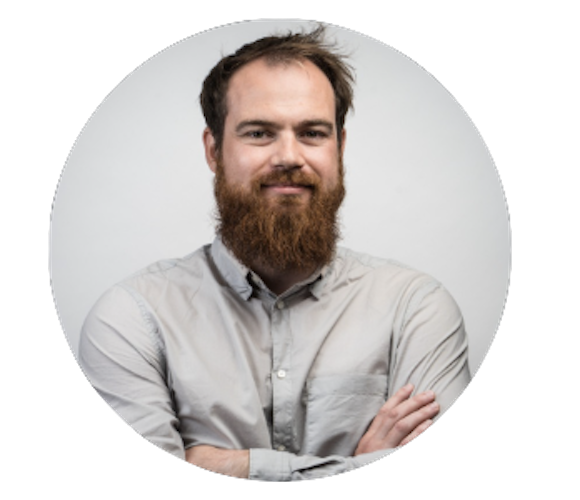
\includegraphics[width=\linewidth]{static/profilePicture.png}	%trimming relative to image size

%---------------------------------------------------------------------------------------
%	META SKILLS
%----------------------------------------------------------------------------------------
            \cvsection{SKILLS}

            \cvskill{Javascript} {7+ yrs} {1} \\[-2pt]

            \cvskill{NodeJs} {7+ yrs} {1} \\[-2pt]

            \cvskill{React} {4+ yrs} {0.70} \\[-2pt]

            \cvskill{Typescript} {4+ yrs} {0.70} \\[-2pt]

            \cvskill{Serverless} {3+ yrs} {0.5} \\[-2pt]

            \cvskill{GraphQl} {3+ yrs} {0.5} \\[-2pt]

            \cvskill{GIT} {7+ yrs} {1} \\[-2pt]

            \cvskill{BDD (Sql,NoSql)} {7+ yrs} {1} \\[-2pt]


            \vfill\null
            \cvsection{CONTACT}

            \icontext{MapMarker}{12}{Brest, Paris}{black}\\[6pt]
            \icontext{MobilePhone}{12}{+33 (0)6 88 03 29 37}{black}\\[6pt]
            \iconemail{Envelope}{12}{roland.paire@gmx.fr}{roland.paire@gmx.fr}{black}\\[6pt]
            \iconhref{Linkedin}{12}{roland-paire}{rhttps://www.linkedin.com/in/roland-paire/}{black}\\[6pt]

            \vfill\null
            \cvqrcode{0.7}

%---------------------------------------------------------------------------------------
%	EDUCATION
%----------------------------------------------------------------------------------------
            \newpage
            \cvsection{\'Etudes}

            \cvmetaevent
            {2012 - 2013}
            {Master de comp\'{e}tence compl\'{e}mentaire en informatique}
            {Universit\'e de Rennes 1}
            {Cours principaux : Introduction \`a la programmation ({\em caml}), Programmation 1 et 2 ({\em Java}), Conception Web ({\em HTML, CSS, PHP, JavaScript, Ajax}), Algorithme 1 et 2 ({\em C++}), {\em XML}, Langage {\em C}, {\em C++}, Analyse ({\em UML}), Syst\`eme 1 et 2 ({\em Assembly, Java}), Base de donn\'ees ({\em MySql}), caor.}

            \cvmetaevent
            {2010 - 2012}
            {Master de mod\'elisation de syst\`emes biologique}
            {Universit\'e de Rennes 1}
            {Cours principaux : Programmation ({\em Python}), Algorithme ({\em Scilab}), Dynamiques de population ({\em R}), Maths : statistiques, probabiliti\'es, Analyse de sensibilit\'e, mod\`ele SIR, \'Epid\'emiologie.}

            \cvmetaevent
            {2007 - 2010}
            {Licence de biologie cellulaire et physiologie}
            {Universit\'e de Bretagne Occidentale}
            {Cours principaux : Physiologie, G\'en\'etique, Maths, Bioinformatique (Tests Statistiques), Biochimie, Biologie Mol\'eculaire, Biologie Marine, Biologie V\'eg\'etale et Animale, Biotechnologie, Dynamiques de population.}

            \vfill\null
            \cvqrcode{0.7}

        \end{leftcolumn}
        \begin{rightcolumn}
%---------------------------------------------------------------------------------------
%	TITLE  HEADER
%----------------------------------------------------------------------------------------
            \fcolorbox{white}{darkcol}{\begin{minipage}[c][3.5cm][c]{1\mpwidth}
                                           \begin {center}
                                               \HUGE{ \textbf{ \textcolor{white}{ \uppercase{ Roland PAIRE } } } } \\[-18pt]
                                               \textcolor{white}{ \rule{0.1\textwidth}{1.25pt} } \\[4pt]
                                               \large{ \textcolor{white} {S\'enior D\'eveloppeur fullstack - Freelance} }
                                           \end {center}
            \end{minipage}} \\[12pt]
            \vspace{0pt}

%---------------------------------------------------------------------------------------
%	PROFILE
%----------------------------------------------------------------------------------------
%            \vfill\null
%            \cvsection{PROFILE}
%
%            \cvtext{IT Consultant with strong theoretical skills and a passion for OpenSource sofware.\\
%
%            DevOps Engineer, specialized both in automation and in custom application development, experienced with large projects and heterogeneous infrastructures. The link between development and operations, comfortable in both.\\
%
%            Customer-oriented and structured method of working, focused on quality and maintainability. Highly motivated to work in a team, both comfortable in big companies as in small teams.\\
%
%            }

%---------------------------------------------------------------------------------------
%	WORK EXPERIENCE
%----------------------------------------------------------------------------------------
%            \vfill\null
            \cvsection{Exp\'erience professionnelle}

            \cvevent
            {Nov 21 - Jan 23}
            {Senior software developer}
            {Heyday by Hootsuite, Montr\'eal, Canada}
            {Développement d’une application pour améliorer la présence web des commerces sur les différents canaux (Messenger, Twitter, Instagram, WhatsApp) via un dashboard pour centraliser tous les canaux et un chatbot sur le site e-commerce.}
            {\cvlist{
                \item Conception d’architecture pour passer d’un monolithe à du micro-service et une API type SaaS
                \item Intégration des logiciels Hootsuite et Heyday
                \item Formation des développeurs sur l’API et le backend Heyday
                \item Maintenance de l'infrastructure exitante
                \item Conception et mise en place des services d’authentification et d’autorisation (SSO)
            }}
            {\cvlist {
                \item NestJs, NodeJs, Micro-service, serverless, SaaS, Gitlab, Typescript, AWS, DynamoDb, Lambda, SQS
                \item OpenAPI, Agile, suivi et planification de projects, étude de faisabilité technique et  de dette technique
            }}

%            \vfill\null
            \cvevent
            {Avr 20 - Nov 21}
            {Backend D\'eveloppeur, freelance}
            {Heyday, Montr\'eal, Canada}
            {Développement d’un chatbot pour améliorer le travail des équipes support et améliorer les ventes sur les sites e-commerce.}
            {\cvlist{
                \item Intégration d’API tierces pour le chatbot {\small(Prestashop, shopify, salesForce, ...)}
                \item Intégration de canaux de communication {\small(Whatsapp, instagram, ...)}
                \item Maintenance et développement des nouvelles fonctionnalités pour le chatbo
                \item Montée en compétence des nouveaux développeurs sur le produit
                \item POC sur de nouvelle technologie
            }}
            {\cvlist {
                \item NodeJs, Typescript, NoSql, cloudformation, AWS, Dynamodb, lambda, IAM, GitLab
                \item Agile, autonomie, analyse fonctionnelle et technique, TDD, rédaction fonctionnelle
            }}

%            \vfill\null
            \cvevent
            {Nov 16 - D\'ec 20}
            {Co-fondateur et CTO}
            {HOTEL SKIPPER, Brest, France}
            {Développement d’une application SaaS de contrôle de gestion pour les hôtels.}
            {\cvlist{
                \item Étude des usages des hôteliers sur la gestion de leurs exploitations
                \item Conception de l’application web et d’une architecture logicielle
                \item Choix des technologies adaptées au projet pour limiter la dette technique
                \item Création d’un POC, et déploiement de versions commercialisables
                \item Mangement d’une équipe de 5 développeurs
                \item Conception d’une architecture Micro-services
                \item Mise en place du déploiement continu avec les tests automatiques (TDD)
            }}
            {\cvlist {
                \item AWS, NodeJs, NestJs, React, Typescript, GraphQl, MongoDB, Github, Météor
                \item Méthode Agile, Conception d'architecture, gestion d'équipe
            }}

            \cvevent
            {Mai 14 - Nov 16}
            {D\'eveloppeur Business Intelligence (BI)}
            {SOPRA STERIA GROUP, Nantes, France}
            {Développement et maintenance d’applications de BI pour le client RTE.}
            {\cvlist{
                \item Réalisations d’études d’impact et de devis
                \item Développement d’application à partir du besoin client maintenance
                \item Maintenance d’application
                \item Formateur sur Informatica et Shell
                \item Lead Développeur
                \item Mise en place d'outils d'automatisation des tests
            }}
            {\cvlist {
                \item ETL Informatica, Java, Javascript, Html/css, Shell, Oracle, SQL, Jenkins
                \item Création et gestion de formation
            }}

            \cvevent
            {Avr 13 - Sep 13}
            {Stage Ingénieur développement}
            {THALES UNDERWATER SYSTEMS, Brest, France}
            {Intelligence artificielle d'un drone sous-marin.}
            {\cvlist{
                \item D\'eveloppement d'un syst\`eme expert en Prolog
                \item Impl\'ementation d'une IA pour trouver la meilleure trajectoire du drone
                \item Mise en place d'un service web en Java
            }}
            {\cvlist {
                \item Prolog, Java, PostgreSql
                \item Algorithme A*
            }}

% hotfixes to create fake-space to ensure the whole height is used
            \mbox{}
            \vfill
            \mbox{}
            \vfill
            \mbox{}
            \vfill
            \mbox{}
        \end{rightcolumn}
    \end{paracol}
\end{document}
